\documentclass{article}
\usepackage{graphicx}
\usepackage{algpseudocodex}
\usepackage{amsmath}
\usepackage{amssymb}
\usepackage{listings}
\usepackage{color}

\renewcommand{\ttdefault}{pcr}
\lstset{ 
    basicstyle=\color{black}\ttfamily,
    keywordstyle=\color{purple}\bfseries,
    commentstyle=\color{gray},
    numberstyle=\color{lightgray},
    stringstyle=\color{blue},
    identifierstyle=\color{brown},
    escapeinside={\`}{\`},
    breakatwhitespace=false,
    breaklines=true,
    extendedchars=true,
    keepspaces=true,
    numbers=left,
    showspaces=false,
    showstringspaces=false,
    showtabs=false,
    tabsize=8,
    title=\lstname,
}

\title{Crazy Quines}
\author{Maxwell Tang}
\date{Due 10 May 2024}

\begin{document}
\maketitle
Okay, so we've just received our first message from the great unknown,
    and it looks like the strangers from another world have another world have something to share with us!
After decoding the message we wait to see what it is. \vspace*{0.25cm}
\\Maybe it's a polynomial time solution for 3-SAT.
\\Maybe it's a proof of the Goldbach conjecture.
\\Maybe it's a computer virus that destroys our planet.
\bigbreak
It's a JavaScript/TypeScript runtime.
\bigbreak
Well this is a little disappointing, but we still want to communicate with our peers from another planet.
In particular, it would be nice to prove our intelligence to them, so that they don't get any funny ideas!
To do this, we can send a computer program back to them, and to show off our decoding skills, we could write it in TypeScript.
We don't know what kinds of programs would be interesting to them, but quines seem like a good candidate for such a "universally interesting" program.
The problem is, though, that these guys are thousands of light-years away!
There's no way that our signal is getting to them intact.
Thus, we would like our program to be self-healing: it always returns the original code even when a character is dropped.

Well, that's enough with the intro, let's work on a quine!
In all quines, a common 








\section*{Examples!}

\subsection*{Equations}
$$\int_{0}^{\pi}\sin x dx = 2$$

\subsection*{Diagrams}
\begin{center}
    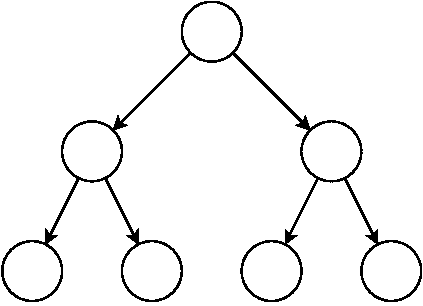
\includegraphics[width=0.5\textwidth]{example-figure.pdf}
\end{center}

\subsection*{Algorithms}
\begin{algorithmic}
    \Function{factorial}{n}
        \State x := 1
        \ForAll{i from 1 to n}
            \State x := x * i
        \EndFor
        \State \Return x
    \EndFunction
\end{algorithmic}

\subsection*{Code}
\lstinputlisting[language=C]{example-code.c}
\end{document}
